\documentclass{llncs}
\bibliographystyle{splncs}
\usepackage{hyphenat}
\usepackage{amssymb}
\usepackage{floatrow}
\setcounter{tocdepth}{3}
\usepackage{graphicx}
\graphicspath{ {./bilder/} }
\usepackage{wrapfig}
\usepackage{epstopdf}
\usepackage{listings}
\usepackage{url}
\usepackage{xcolor}
\usepackage{amsmath}
\usepackage{caption}
\usepackage{hyperref}
\captionsetup[figure]{font=small}
\newcommand{\keywords}[1]{\par\addvspace\baselineskip
\noindent\keywordname\enspace\ignorespaces#1}
\lstset{ 
	numbers=left,
 	firstnumber=1,
 	numberfirstline=true
}
\begin{document}

\hypersetup{
    colorlinks=true,
    linkcolor=blue,
    filecolor=magenta,      
    urlcolor=cyan,
    bookmarks=true,
    pdfpagemode=FullScreen,
}
\mainmatter  % start of an individual contribution

% first the title is needed
\title{Report on the Project\newline"Multi-Agent Path Finding"}

% a short form should be given in case it is too long for the running head
\titlerunning{}

% the name(s) of the author(s) follow(s) next
%
% NB: Chinese authors should write their first names(s) in front of
% their surnames. This ensures that the names appear correctly in
% the running heads and the author index.
%
\author{Marcus Funke (Mat.Nr.787912), Maximilian Wiedenhöft (Mat.Nr.786868)}
%
\authorrunning{}
% (feature abused for this document to repeat the title also on left hand pages)

% the affiliations are given next; don't give your e-mail address
% unless you accept that it will be published
\institute{Universität Potsdam}

%
% NB: a more complex sample for affiliations and the mapping to the
% corresponding authors can be found in the file "llncs.dem"
% (search for the string "\mainmatter" where a contribution starts).
% "llncs.dem" accompanies the document class "llncs.cls".
%


\maketitle


\begin{abstract}
The use of autonomous agents has become widespread in the field of logistics. The warehouses of tech giants such as Amazon could not function without them anymore. It is therefore of great  importance to identify and tackle the technical issues these robots face. To that end, our work was focused on creating a tool that allows for the seamless merging of plans of individual robots.\newline
Section 1 is a short introduction to the background of our project and a first look at the concrete issue we were tasked with solving. In the second section we briefly talk about the basic make up of the program files we worked on, before explaining in detail the functionalities of our merger in section 3 and how it deals with a variety of problems in section 4.\newline
The report concludes with a comparison of our work with that of four other groups working on the same project in the 5th section, before finishing up with an outlook on our future plans in section 6.
\end{abstract}
\tableofcontents

\section{A short introduction to asprilo and Multiple Agent Path Finding}

Two specific terms need explaining in order to fully understand the work done by our group. The first of these is asprilo.\newline\newline 
asprilo was born of the need for complex benchmarking in the field of answer set programming. It is a benchmark environment consisting of four distinct parts: a benchmark generator, a checker for solutions, a visualization tool for both benchmarks and solutions and finally a variety of reference encodings. It allows for the creation of scalable, standardized benchmark suites, their visualizations, both with and without solution, and for checking their correctness via the modular solution checker.\newline
The goal of asprilo is to create abstractions of intra-logistics systems in a warehouse environment. It involves multiple robots, shelves (which may or may not contain ordered products) and picking stations, to which robots may deliver shelves containing products. Per unit of time, a robot may perform exactly one out of a list of possible actions, such as moving or delivering shelves. \newline\newline
A set of restrictions further dictates what a robot may or may not do. For example, as they are supposed to represent solid objects in a real world scenario, no more than one robot is allowed to occupy the same square at the same time, nor are they allowed to move "through" one another to switch positions. A number of different asprilo domains exist, with both the M and B Domain being of importance for this report. \newline
In the A domain, each robot receives an order for a certain number of copies of a product from a picking station, navigates to a shelf containing this product to pick up, moves with the shelf to the picking station and then delivers exactly the number of products requested. It takes into account how much of a product is on a shelf and how much of it remains after delivery. The robot then returns the shelf to the storage area.\newline
The B domain simplifies this process by not asking for a specific quantity of a product, only that it is present on a shelf. It also does not remove the product from the shelf during delivery.\newline\newline
The M domain is another simplification. Here, all that is asked of a robot is that it moves under a shelf with an ordered product. Once it has done so, its work is over. picking stations are done away with, as is the need for a robot to pick up and put down shelves or deliver products. This domain exists specifically to help with parallel planning and Multi-Agent Path Finding. As such, it is the domain we spent the most time working in.\newpage
The second term requiring explanation is aforementioned Multi-Agent Path Finding, or MAPF. It concerns itself with the issue of how to successfully merge the pre-generated plans of two or more autonomous agents in a timely manner. Its main issue arises from the fact that said agents all act concurrently, and collisions between them are likely and need to be dealt with in order to successfully create a working merged plan.
\begin{figure}[h!]
\floatbox{figure}[\FBwidth]
{\caption{An example of a warehouse environment. Green and blue circles denote shelves, red and yellow boxes denote robots. The highway upon which robots may move is shown as blue squares, while the striped yellow square marks the location of the picking station.}\label{fig:test}}
{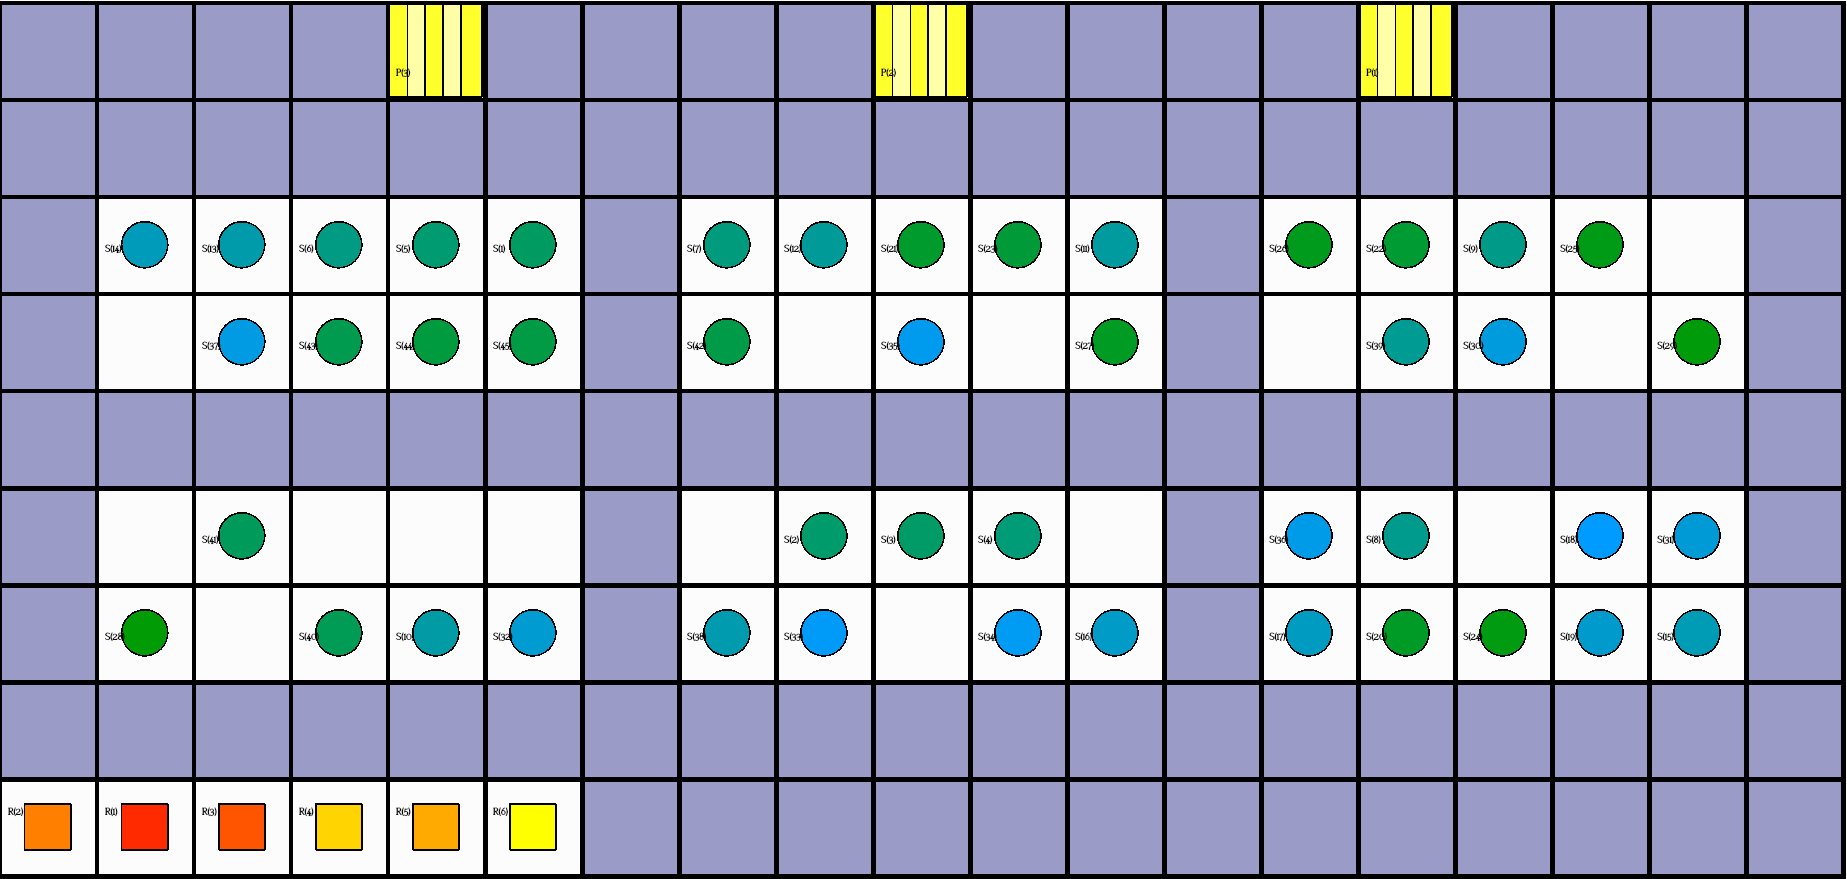
\includegraphics[width=\textwidth, height= 5cm, keepaspectratio]{asp}}
\end{figure}\newpage



\section{Preliminaries}
We based our work on the files provided in the asprilo-encodings by potassco. Specifically, we worked on action-M.lp and action-MPP.lp. Furthermore, our merger requires input.lp, output.lp and goal-M.lp/goal-B.lp in order to operate. This chapter will contain short explanations on what each of these encodings is used for and how we began our work.
\subsection{action-M.lp and action-MPP.lp}

\begin{lstlisting}[basicstyle=\fontsize{9}{11}\selectfont\ttfamily,frame=single,breaklines=true]
time(1..horizon).

direction((X,Y)) :- X=-1..1, Y=-1..1, |X+Y|=1.
nextto((X,Y),(DX,DY),(X',Y')) :- direction((DX,DY)), position((X,Y)), position((X',Y')), (X,Y)=(X'-DX,Y'-DY), (X',Y')=(X+DX,Y+DY).

{ move(R,D,T) : direction(D) } 1 :- isRobot(R), time(T).

% - move/3
position(R,C,T) :- move(R,D,T), position(R,C',T-1),     nextto(C',D,C).
                :- move(R,D,T), position(R,C ,T-1), not nextto(C ,D,_).

% - inertia 
position(R,C,T) :- position(R,C,T-1), not move(R,_,T), isRobot(R), time(T).

% - edge collision
moveto(C',C,T) :- nextto(C',D,C), position(R,C',T-1), move(R,D,T).
 :- moveto(C',C,T), moveto(C,C',T), C < C'.
% - vertex collision
 :- { position(R,C,T) : isRobot(R) }  > 1, position(C), time(T).
% - auxiliaries 
 :- { position(R,C,T) } != 1, isRobot(R), time(T).
\end{lstlisting}
From action-M.lp we directly took the definitions of direction/1 (defining movement on a board of squares in either a vertical or horizontal direction), nextto/3 (which checks whether two squares on a grid are neighbours), as well as position/3 (which lets a robot be on a given position as long as said position was reachable in a direction from the previous square the robot occupied, as well as let it simply stand around). \newline
We also adopted its integrity constraints dealing with both vertex and edge collision, as we (rightly) believed them to be of use in debugging our merger. Move/3 is the only element of action-M.lp we scrapped and replaced, as our goal was to make the robots follow predetermined plans to their completion, rather than come up with their own in the instance.\newline\newline
Additionally, when we moved to make our merger compatible with the B-Domain, we took certain elements of the action-MPP.lp as well. The full extent of the action-MPP.lp can be found on the asprilo github provided by potassco, we will only focus on those parts we adapted into our own merger.


\begin{lstlisting}[basicstyle=\fontsize{9}{11}\selectfont\ttfamily,frame=single,breaklines=true]
{move(R,D,T) : direction(D) ;
pickup(R,S,T) : isShelf(S) ;
putdown(R,S,T) : isShelf(S) } 1 :- isRobot(R), time(T).

 carries(R,S,T) :- pickup(R,S,T).
                :- pickup(R,S,T), carries(R,_,T-1).
                :- pickup(R,S,T), carries(_,S,T-1).
                :- pickup(R,S,T), position(R,C,T-1), not position(S,C,T-1).
                :- pickup(R,S,T), position(S,C,T-1), not position(R,C,T-1).

% - putdown/3
               :- putdown(R,S,T), not carries(R,S,T-1).

% - inertia
carries(R,S,T) :- carries(R,S,T-1), not putdown(R,S,T),	    time(T).

% - (in)direct effects
position(S,C,T) :- position(R,C,T  ), carries(R,S,T).
position(S,C,T) :- position(S,C,T-1), not carries(_,S,T), isShelf(S), time(T).

% - vertex collision 
 :- { position(S,C,T) : isShelf(S) }  > 1, position(C),	    time(T).

% - auxiliaries 
 :- { position(S,C,T) } != 1, isShelf(S), time(T).
 :- { carries(R,S,T) } > 1, isRobot(R), time(T).
 :- { carries(R,S,T) } > 1, isShelf(S), time(T).
\end{lstlisting}
Carries/3 helps with identifying which robot is carrying what shelf at what time, and its integrity constraints forbid robots which already carry another shelf from picking up a new one without having put down their own. They also ensure any one shelf is only carried by one robot at any given time, and that a robot must be in the same position as the shelf if it wants to pick it up. A robot may also not put down a shelf if it is not carrying one at all.
\newline
pickup/3 and putdown/3 allow a robot to, instead of making a movement, pick up a shelf they are under or put down a shelf they are carrying, as defined by carries/3. Of course, a robot may still only try and put down a shelf they are actually carrying.\newline
All other additions of action-MPP.lp are merely expansions of already explained features of the old action-M.lp. As such a robot may hold position if carrying a shelf, and only one shelf may occupy the same square at any given time. It also follows logically, that a shelf being carried shares its position with the robot carrying it, and if it is not being carried it will remain in place until picked up.\newline
As before, we scrapped the existing definitions of move/3, pickup/3 and putdown/3, as will be outlined in chapter 3.\newline\newline
Shown so far are merely the original action.lp files. On their own, they were already capable of calculating solutions for pre-generated instances within either the M or B domain, meaning  instances in which all robots, shelfs, picking stations etc. are present, but no external plans are fed into the solver; they are generated on the instance itself with all other robots already in mind. Our goal however was to create a merger able to successfully combine externally created plans of each robot, and make them work in tandem on the instance. By importing the plans of individual robots instead of generating one unified plan on the instance itself, collisions between robots become a threat to the satisfiability of the merged plan.\newline
How we dealt with this problem will be explained in detail in section 4.

\subsection{input.lp}
The file input.lp contains a multitude of definitions, such as what robot(R), shelf(S) or position((X,Y)) mean. It takes this information straight from a generated instance and translates it for easier use by a programmer. As we have made no changes to the file itself and seeing that it is somewhat large, we refrain from providing a copy here and would instead direct you the \hyperlink{thesentence}{potassco github}.

\subsection{output.lp}

The main purpose of output.lp is to convert certain actions (namely move/3, pickup/3 and putdown/3) into a format the vizualiser is able to process correctly. For this purpose it also generates the initial situation in an instance. Note that output.lp is not strictly necessary for our merger to work, but it allows for vizualisation and helps with debugging.

\subsection{goal.lp}\hfill\\
The last and, after the action.lps, perhaps most important files our merger needs are the goal conditions, signified with goal-M.lp and goal-B.lp. Two distinct goal conditions are necessary, as our merger is currently able to solve problems in both the M as well as the B domain. Whether a problem is solvable in the M or B domain is therefore dependent on which goal condition is applied.
\subsubsection{Groundwork}\hfill\\
\begin{lstlisting}[basicstyle=\fontsize{9}{11}\selectfont\ttfamily,frame=single,breaklines=true]
:- ordered(O,A), not processed(A).
:- not position(S,C,horizon), position(S,C,0), isShelf(S).
:- carries(_,_,horizon).
\end{lstlisting}
As both goal conditions require these constraints, we will examine them first. Line 1 is to ensure that any product which was ordered gets processed. What exactly it means to be processed will depend on the domain. Line 2 posits that shelves have to be in the exact same position at the end of the program as they were at the start, meaning they are to be returned to their storage positions. Finally, line 3  demands that robots do not carry any shelf at the end of the program. If any of these integrity contraints is violated, the found plan will not be considered valid and be scrapped instead.
\subsubsection{goal-M.lp}\hfill\\
The goal-M.lp defines the goals specifically for the M domain. It looks as follows:
\begin{lstlisting}[basicstyle=\fontsize{9}{11}\selectfont\ttfamily,frame=single,breaklines=true]
processed(A,R) :- ordered(O,A), shelved(shelf(S),A), isRobot(robot(R)),position(shelf(S),C,0), position(robot(R),C,horizon), R=S.
processed(A)   :- processed(A,R).
\end{lstlisting}
Line 1 defines what it means for an attribute A to be processed. Specifically, every shelf which contains an ordered product requires a robot present under it at the end of the program. Line 2 shortens it from processed/2 to processed/1, in order to fit the integrity constraints mentioned above. Note that the robot present under the shelf needs to share that shelf's ID. This was done for the purpose of simplification, as it was easier in terms of logistics and clarity to have robot 1 be assigned shelf 1 and so on.

\subsubsection{goal-B.lp}\hfill\\
goal-B.lp meanwhile contains the goal conditions for the B domain. It is somewhat more extensive than goal-M.lp, though not by much.
\begin{lstlisting}[basicstyle=\fontsize{9}{11}\selectfont\ttfamily,frame=single,breaklines=true]
serves(S,P):- position(R,C,T), carries(R,S,T), position(P,C).
process(O,A) :- ordered(O,A), target(O,P), shelved(S,A), serves(S,P).
processed(O) :- process(O,_).
:- position(_,C,horizon), position(_,C).
\end{lstlisting}
Notice Line 1, which defines the predicate serves/2 so as to refer to a robot carrying a shelf while standing on a picking station. This aides the new definition of process/2, which is satisfied if a shelved ordered product was served at the picking station that requested the product. Line 3 again serves to minimize the predicate. The constraint of line 4 now demands that nothing, neither robot nor shelf, shares a space with a picking station at the end of the program, so as to avoid blockage.\newpage


\section{Basics of the Merger}

Outlined in this chapter is the general groundwork which was needed to allow our merger to perfom its functions, starting with the override of the old movement rule with a new one.
\subsection{Importing the plans}
\begin{lstlisting}[basicstyle=\fontsize{9}{11}\selectfont\ttfamily,frame=single,breaklines=true]
step_move(robot(R),D,T,0) :- plan_occurs(object(robot, R), action(move,D), T).
step_pickup(robot(R),shelf(S),T,0) :- plan_occurs(object(robot, R), action(pickup,object(shelf,S)), T).
step_putdown(robot(R),shelf(S),T,0) :- plan_occurs(object(robot, R), action(putdown,object(shelf,S)), T).
\end{lstlisting}
Each single step of a plan is simply called plan\_occurs/3. Our merger requires, independent of domain, all movements generated by a robot's plan, saving them in a "blue print" called step\_move/4, with which it will continue working from then on out. In domains other than M, it also copies over all pickups and putdowns a robot is supposed to carry out, saved in step\_pickup/4 and step\_putdown/4, respectively.\newline
\subsection{The Collision Depth}
Next we decided to implement a variable we call the collision depth.
\begin{lstlisting}[basicstyle=\fontsize{9}{11}\selectfont\ttfamily,frame=single,breaklines=true]
collision(R,0,0) :- isRobot(R).
collision(R,T+1,N) :- collision(R,T,N), not collision(R,T+1,N+1), horizon>T.
\end{lstlisting}
The general idea of collision/3 is to provide us with a tool that generates and keeps track of the correct collision depth at any one time for each individual robot. As seen in Line 2, the collision depth of each robot begins at 0 at the start of the program, before any move has been made. Line 3 ensures that the collision depth N remains constant for a robot from one time step to the next, so long as it is not involved in a collision at that time. This means a robot which does not encounter a collision throughout a benchmark ends with zero collisions.\newline\newline
Of course, such a situation is unlikely and not very interesting to consider. Therefore variants for each collision type also exist.\newpage
\begin{lstlisting}[basicstyle=\fontsize{9}{11}\selectfont\ttfamily,frame=single,breaklines=true]
collision(R,T,N+1) :- wait(R,T), collision(R,T-1,N), horizon>T.
collision(R,T,N+1) :- dodge_who(R,_,T), collision(R,T-1,N), horizon>T.
collision(R,T,N+1) :- s_coll(R,T), collision(R,T-1,N), horizon>T.
collision(R,T,N+1) :- nmc_dodge(R,T), collision(R,T-1,N), horizon>T.
\end{lstlisting}
Line 1 increases the collision depth of a robot whenever it loses priority in a vertex collision, meaning it had to wait. Line 2 meanwhile serves to increment the collision depth for robots which lose out in edge collisions, where they were forced to dodge out of the way. Line 3 covers a situation not naturally occurring in the M Domain, since it involves the collision of a robot carrying a shelf with a stationary shelf, which may only occur in A, B and C. Finally, Line 4 increments the collision depth for a collision in which a robot becomes unable to return to a spot they dodged from.\newline
\subsection{B Domain Updates}
\subsubsection{carries/3}\hfill\\
Certain changes and updates had to be made to get carries/3 to work as we wanted it to.
\begin{lstlisting}[basicstyle=\fontsize{9}{11}\selectfont\ttfamily,frame=single,breaklines=true]
carries(R,S,T)  :- carries(R,S,T-1), not putdown(R,S,T), isRobot(R), isShelf(S), time(T).
\end{lstlisting}
To that end we added a recursive element to the definition of carries. This way, a robot will remember that it carries a shelf by checking that it carried a shelf in the last step and has no order to put it down in this step.
We then updated the original definition of carries/3.
\begin{lstlisting}[basicstyle=\fontsize{9}{11}\selectfont\ttfamily,frame=single,breaklines=true]
carries(R,S,T)  :- pickup(R,S,T), time(T), position(R,C,T-1), position(S,C,T-1).
\end{lstlisting}
Our aim was to ensure that within the definition of carries it is explicitly known that only a robot which shares the square with the shelf is able to start carrying the shelf.

\subsubsection{putdown/3}\hfill\\
The predicate putdown/3 had be updated to fit our expectations as well.
\begin{lstlisting}[basicstyle=\fontsize{9}{11}\selectfont\ttfamily,frame=single,breaklines=true]
:- putdown(R,S,T), position(R,C,T-1), position(_,C).
:- putdown(R,S,T), position(R,C,T-1), highway(C).
\end{lstlisting}
We added two additional integrity constraints in order to prevent robots from putting down their shelf on the square of a picking station (Line 1), as well as prevent them from simply putting them down on a highway square (Line 2). Combined with the integrity constraints of the goal condition we can therefore guarantee that any uncarried shelf that is stationary will only ever be standing on its original spot in a warehouse.
\subsection{Groundworks for the Merging of Plans}
Last part of our groundwork are two additional types of move actions, move/3 and move/4, as well as the new pickup/3 and putdown/3.
\begin{lstlisting}[basicstyle=\fontsize{9}{11}\selectfont\ttfamily,frame=single,breaklines=true]
move(R,D,T,N) :- step_move(R,D,T,N), collision(R,T-1,N).

move(R,D,T) :- move(R,D,T,N), not wait(R,T), not dodge_who(R,_,T), not s_coll(R,T), not nmc_dodge(R,T), not putdown(R,_,T), not pickup(R,_,T).
\end{lstlisting}
move/4 exists purely so as to make sure the merger only considers the current step\_move/4 with the highest collision depth for the final act of merging. Meanwhile, the new move/3 takes these movement actions as input, granted they are not occurring at the same time as a waiting period, one of the two dodging motions, a pickup, putdown or a shelf collision, for all of these are added to the final plan seprately, as will be discussed in the appropriate sections.
\begin{lstlisting}[basicstyle=\fontsize{9}{11}\selectfont\ttfamily,frame=single,breaklines=true]
pickup(R,S,T) :- step_pickup(R,S,T,N), collision(R,T-1,N).
putdown(R,S,T) :- step_putdown(R,S,T,N), collision(R,T-1,N).
\end{lstlisting}
Finally, pickup/3 and putdown/3 are also imported into the final plan, as the B domain expects a robot to be able to interact with shelves, meaning picking them up, carrying them to picking stations and back and putting them down again. As such, the final plan needs to be able to reflect that.\newline\newline
As a last modification we saw as necessary, we allow any robot which has successfully completed its plan to move as it will. This movement will still be restricted by the specifics given in the goal condition, so any final merged plan in which robots would move away from the square they ought to be on (M domain) or any actions involving the unscheduled moving of shelves (B domain) will simply be thrown out.


\begin{lstlisting}[basicstyle=\fontsize{9}{11}\selectfont\ttfamily,frame=single,breaklines=true]
{move(R,D,T,N) : direction(D);
pickup(R,S,T) : isShelf(S), not step_pickup(R',S,T',_), R'!=R, isRobot(R'), T'>T, time(T');
putdown(R,S,T) : isShelf(S)} 1 :- isRobot(R), time(T), not step_move(R,_,T,N), not step_pickup(R,_,T,N), not step_putdown(R,_,T,N), collision(R,T-1,N).
\end{lstlisting}
As you can see, a robot may only pick up a shelf if that shelf is not supposed to be picked up by another robot at a later time, nor is it allowed to put down a shelf or move freely as long as there exist moves that are still assigned to it, be they movement actions (as represented by step\_move/4) or shelf interactions (represented by step\_pickup/4 and step\_putdown/4).

\section{Collisions}
This chapter will deal with the variety of collisions which we found to occur in our benchmarks, beginning with the generalized vertex and edge collision, before expanding into more fringe cases. Then those collisions which occur outside the M Domain, involving shelves, will be described. Along with each type of collision we will detail how the merger is meant to deal with it.
\subsection{Vertex Collisions}
A vertex collision is an occurrence, in which two different robots attempt to move to the same, third square in the same time step. This situation is shown in figure 1. 
Our solution to this simple problem is as follows.
\begin{lstlisting}[basicstyle=\fontsize{9}{11}\selectfont\ttfamily,frame=single,breaklines=true]
wait(R2,T) :- move(R1,D1,T,N1), move(R2,D2,T,N2), position(R1,C1',T-1), N1>N2, nextto(C1',D1,C), position(R2,C2',T-1), nextto(C2',D2,C), not dodge_who(R2,_,T), not wait(R1,T).
wait(R2,T) :- move(R1,D1,T,N), move(R2,D2,T,N), position(R1,C1',T-1), R2>R1, nextto(C1',D1,C), position(R2,C2',T-1), nextto(C2',D2,C), not dodge_who(R2,_,T), not dodge_who(R1,_,T), not no_dodge(R2,T).
\end{lstlisting}
The rule wait/2 is written in such a way that it checks if the above described situation arises, by simply comparing where the movement actions of each individual robot would take them.
Should they end up at the same square at the same time, wait/2 then tries to identify which robot should be given priority to keep moving, and which has to stop.


\begin{wrapfigure}[16]{r}{5cm}
    \centering
    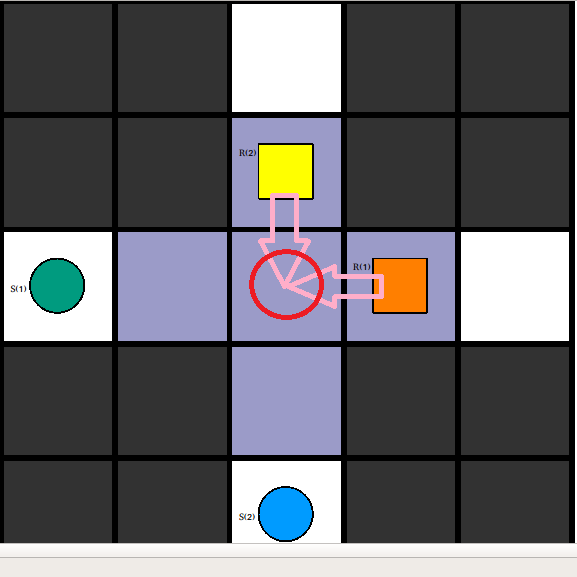
\includegraphics[width=5cm,height=5cm,keepaspectratio]{vertex}

\caption{Example of a vertex collision}
\end{wrapfigure}
It does so by first comparing the collision depths of both robots, with the robot with a lower depth being told to wait, as seen in Line 1, then by comparing their IDs should a tie breaker be necessary. This is shown in Line 2. In such a case, the robot with the higher ID will be assigned to wait.\newline
Important to note is that a robot is only eligible to wait, if it is not the dodging robot in an edge collision at the same time (not dodge\_who(R2,\_,T)). It may also not carry out a wait move if the other robot in the vertex collision is already waiting as well (not wait(R1,T)), nor may a robot wait if its opponent is forced to dodge at the same time (not dodge\_who(R1,\_,T)). Lastly, if a robot is in an edge collision but unable to dodge at all, it may also not wait (not no\_dodge(R2,T)). no\_dodge/2 and dodge\_who/3 will defined in the next chapter.\newline
\begin{figure}[h!]
\floatbox[{\capbeside\thisfloatsetup{capbesideposition={right,top},capbesidewidth=4cm}}]{figure}[\FBwidth]
{\caption{Seen here a situation in which the lead robot of a convoy is forced to wait by robot 1. It now blocks the square robot 3 intended to move to. The new variant of wait/2 now checks for this eventuality and forces robot 3 to wait until the square is free of robot 2.}\label{fig:test}}
{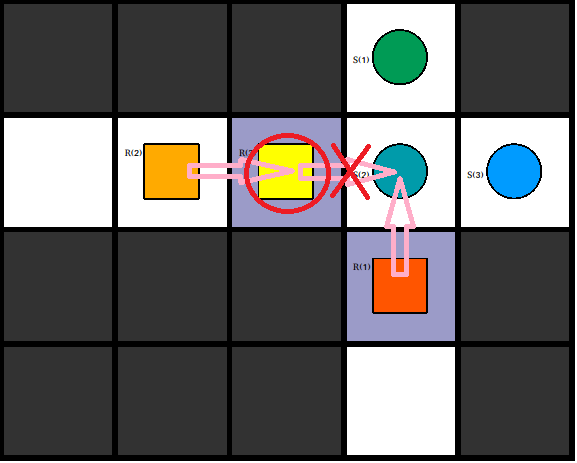
\includegraphics[width=\textwidth, height= 5cm, keepaspectratio]{convoy}}
\end{figure}\newline
Related to the vertex collision, but not a "true" vertex collision itself, is a situation in which a convoy of robots moving in a line is held up and forced to wait. To allow robots beyond the lead robot to wait, the following addition to the wait rule became necessary. A situation like this is illustrated in Figure 2.
\begin{lstlisting}[basicstyle=\fontsize{9}{11}\selectfont\ttfamily,frame=single,breaklines=true]
wait(R2,T) :- move(R2,(DX,DY),T,N), position(R2,C2',T-1), nextto(C2',(DX,DY),C), position(R1,C,T-1), wait(R1,T), not move(R1,(-DX,-DY),T,_).
\end{lstlisting}
This variant of wait/2 no longer checks whether or not two robots wanted to enter the same square at the same time, but rather if the square a robot is trying to move to is currently occupied by a robot which has been assigned to wait in this time step. If this is the case, it also gets assigned the command to wait.\newline\newline
One additional condition must be true for this rule to trigger: The waiting robot R1 must not be trying to move opposite the direction of the new waiting robot R2, as that would end up causing issues with the handling of edge collisions. This addition is necessary in order to avoid mixups in multi-robot collisions of mixed collision type.\newline\newline
So far we have merely instituted new rules to be considered by the merger. The modification of a robot's plan happens with the following step.
\begin{lstlisting}[basicstyle=\fontsize{9}{11}\selectfont\ttfamily,frame=single,breaklines=true]
step_move(R,D,T1+1,N+1) :- step_move(R,D,T1,N), wait(R,T), collision(R,T-1,N),(T1+1)>T, horizon>T1.
step_pickup(R,S,T1+1,N+1) :- step_pickup(R,S,T1,N), wait(R,T), collision(R,T-1,N),(T1+1)>T, horizon>T1.
step_putdown(R,S,T1+1,N+1) :- step_putdown(R,S,T1,N), wait(R,T), collision(R,T-1,N),(T1+1)>T, horizon>T1.
\end{lstlisting}\newpage
As previously explained, step\_move/4 contains the movement of each robot for each time step and collision depth. When a robot is told to wait in a time step T, any move of that robot which would happen during or after time T is shifted back by one unit of time, with its collision depth being incremented by one as well. The same happens for both pickup and putdown actions. Finally, recall the following line of code from the previous chapter.
\begin{lstlisting}[basicstyle=\fontsize{9}{11}\selectfont\ttfamily,frame=single,breaklines=true]
move(R,D,T) :-  move(R,D,T,N), not wait(R,T), not dodge_who(R,_,T), not s_coll(R,T), not nmc_dodge(R,T), not putdown(R,_,T), not pickup(R,_,T).
\end{lstlisting}
Remember that move/3 is what the output will return as the occurs/3 for each robot, to be read by the vizualiser. Remember further that move/4 is a copy of each step\_move/4 of each robot for each unit of time with the highest collision depth. If a robot has been told to wait, all of its moves from that point on will be shifted to occur one step in time late. The move it was inteded to complete at the time the wait was triggered is deleted, as it is not supposed to do anything at that moment.\newline
In other words, the final plan simply has no order at all for that robot in the specified time step, which makes it stand around and do nothing at all, which is equivalent to waiting a turn.

\subsection{Edge Collisions}
The second collision type we will deal with is the edge collision. In it, two different neighbouring robots attempt to switch their positions in one move. As they are meant to be abstractions of solid objects, this causes a problem, as they are unable to simply phase through one another, and one will have to move out of the way for the other to pass. In other words, we needed to introduce the concept of dodging. 
\begin{lstlisting}[basicstyle=\fontsize{9}{11}\selectfont\ttfamily,frame=single,breaklines=true]
dodge_coll(R1,R2,T) :- move(R1,D1,T,N1), move(R2,D2,T,N2), position(R1,C1,T-1), R2>R1, nextto(C1,D1,C2), position(R2,C2,T-1), nextto(C2,D2,C1).
\end{lstlisting}
In order to detect when such a collision occurs, we created the rule dodge\_coll/3. All it does is check for two neighbouring robots, R1 and R2, if the movement action of R1 would put it on the square held by R2, if the movement action of R2 would put it on the square held by R1, and if these two actions would occur in the same time step T. \newline Should this be the case, the merger notes down this occurrence. In order to avoid duplicate notations of the same collision (as a collision between R1 and R2 is essentially equivalent to a collision between R2 and R1), only the version in which the robots are ordered by numerically ascending ID is registered. This has the side effect that several later rules connected to dodge\_coll/3 have to be written twice to cover all possible bases. For the time being, we consider this a fair trade off.\newpage
\subsubsection{The basic dodge move}\hfill\\
Having detected an edge collision, the merger needs to be able to detect where a robot might feasibly dodge to. For this purpose, dodge\_where/3 was written.
\begin{lstlisting}[basicstyle=\fontsize{9}{11}\selectfont\ttfamily,frame=single,breaklines=true]
dodge_where(R1,D,T) :-  dodge_coll(R1,R2,T), direction(D), nextto(C1,D,C1'), position(R1,C1,T-1), position(R2,C2,T-1), C1'!=C2, step_move(R2,D2,T+1,N2), D!=D2, collision(R2,T-1,N2).

dodge_where(R2,D,T) :-  dodge_coll(R1,R2,T), direction(D), nextto(C2,D,C2'), position(R1,C1,T-1), position(R2,C2,T-1), C2'!=C1, step_move(R1,D2,T+1,N1), D!=D2, collision(R1,T-1,N1).
\end{lstlisting}
This rule works by simply searching for any direction D which fulfills the criterion that it leads to an accessible square which is not an intended goal of the opposing robot. Otherwise, the collision between the two would be repeated in the next step and might lead to deadlocks.\newline Of course, the square of the opposing robot itself is also off-limits, as that would obviously be a repeat of the movement actions which caused the edge collision in the first place and not solve anything. Therefore, only directions leading to positions out of the opposing robot's way are considered valid by dodge\_where/3. \newline\newline
Having now determined a direction in which to move, the next step is to decide which robot will be the one to dodge.
\begin{lstlisting}[basicstyle=\fontsize{9}{11}\selectfont\ttfamily,frame=single,breaklines=true]
1{dodge_who(R1,D,T) : dodge_where(R1,D,T)}1 :- dodge_coll(R1,R2,T), N2>N1, collision(R1,T-1,N1), collision(R2,T-1,N2), not no_dodge(R1,T), not no_dodge(R2,T), not back_dodge(R1,T), not back_dodge(R2,T), not occ_dodge(R1,T) .

1{dodge_who(R2,D,T) : dodge_where(R2,D,T)}1 :- dodge_coll(R1,R2,T), N1>=N2, collision(R1,T-1,N1), collision(R2,T-1,N2), not no_dodge(R1,T), not no_dodge(R2,T), not back_dodge(R2,T), not back_dodge(R1,T), not occ_dodge(R2,T).
\end{lstlisting}
dodge\_who/3 was created for this purpose. Like wait/2, it decides by comparing the collision depths of the robots, where again the robot with the lower depth is assigned to dodge, with their IDs serving as tie breakers and the higher ID having to dodge. \newline Then it chooses one of the directions found by the previous rule, dodge\_where/3 for this robot to move in. Predicates no\_dodge/2, back\_dodge/2 and occ\_dodge/2 denote special cases which may occur in an edge collision, each of which gets their own version of dodge\_who/3. As such it is necessary to exclude them in the base version of the rule for it to work and not cause issues in certain specialized benchmarks.\newline\newline
Having decided which robot dodges and where it dodges to, all that remains is to modify the plan of the robot in question.\newpage
\begin{lstlisting}[basicstyle=\fontsize{9}{11}\selectfont\ttfamily,frame=single,breaklines=true]
move(R,D,T) :- dodge_who(R,D,T), collision(R,T-1,N).
step_move(R,(X1,Y1),T+1,N+1) :- dodge_who(R,(-X1,-Y1),T), collision(R,T-1,N), horizon>T.

step_move(R,D,T1+2,N+1) :- step_move(R,D,T1,N), dodge_who(R,_,T), (T1+1)>T, collision(R,T-1,N), horizon>(T1-1).

step_pickup(R,S,T1+2,N+1) :- step_pickup(R,S,T1,N), dodge_who(R,_,T), collision(R,T-1,N),(T1+1)>T, horizon>(T1-1).

step_putdown(R,S,T1+2,N+1) :- step_putdown(R,S,T1,N), dodge_who(R,_,T), collision(R,T-1,N),(T1+1)>T, horizon>(T1-1).

\end{lstlisting}
With line 1 we directly insert the dodge move of a robot into move/3, and thereby into the finalized, merged plan, while line 2 inserts a return move into the individual plan of the robot, by making it move in the opposite direction of the dodge move in the step following the dodge. \newline Finally, all moves of the robot that were to occur from the moment of the edge collision onwards are moved back by 2 steps in the robot's plan in line 4, in order to accomodate the 2 new moves necessary to complete a dodge motion, those being the moving out of the way (dodge) and the associated return move. This of course also applies to actions involving picking up or putting down shelves, as seen in lines 6 and 8.

\subsection{Exceptional Edge Collisions}
It should come as no surprise that a number of exceptional situations may arise when two or more robots collide. Depending on their environment, it may happen that one of them turns out to be unable to dodge anywhere. In more extreme cases, both robots may encounter this issue. Furthermore, with the addition of more robots into a benchmark, multi-robot collisions also become more commonplace, and difficulties between the different rules defined thus far may arise. \newline The following subsections will examine these problems and outline our approach to solve them.

\subsubsection{no\_dodge/2}\hfill\\
The first exception which may occur is that out of two robots encountering each other in an edge collision, one of them is found to be unable to locate "valid" (as defined by dodge\_where/3) spots to move to.\newline
\begin{figure}
\floatbox[{\capbeside\thisfloatsetup{capbesideposition={right,top},capbesidewidth=4cm}}]{figure}[\FBwidth]
{\caption{Seen here is a situation in which robot 3 is stuck in a tunnel and encountering robot 1 in an edge collision (no\_dodge, red circle). Additionally, it encounters robot 2 in a vertex collision at the same time (yellow circle), while robot 1 is blocked from dodging vertically (occ\_dodge).}\label{fig:test}}
{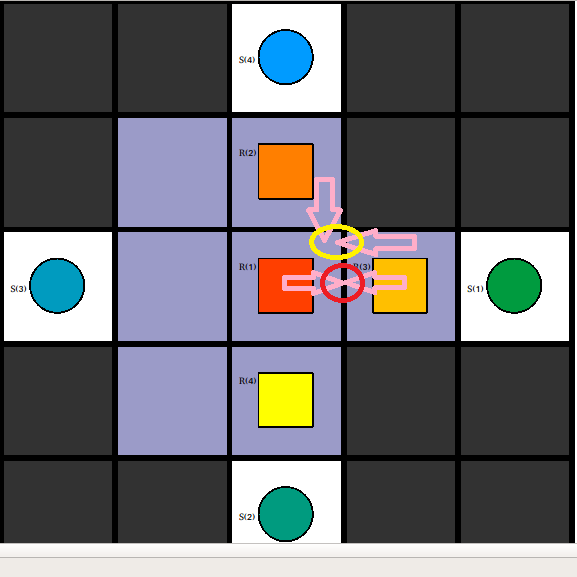
\includegraphics[width=\textwidth, height= 5cm, keepaspectratio]{nododge}}
\end{figure}\newline
Most commonly, this issue arises whenever one of the robots in an edge collision is positioned in the opening of a tunnel, as seen in figure 3, though a collision in the corner of a warehouse also causes it to happen.
For this porpuse, we created the special rule of no\_dodge/2.
\begin{lstlisting}[basicstyle=\fontsize{9}{11}\selectfont\ttfamily,frame=single,breaklines=true]
no_dodge(R1,T) :- not dodge_where(R1,_,T), dodge_coll(R1,R2,T), dodge_where(R2,_,T).
no_dodge(R2,T) :- not dodge_where(R2,_,T), dodge_coll(R1,R2,T), dodge_where(R1,_,T).
:- no_dodge(R,T), dodge_where(R,_,T).
\end{lstlisting}
Lines 1 and 2 ensure, that a robot which is part of an edge collision but is unable to find valid spots to dodge to, while its opponent has no such issue, will now be noted accordingly. Line 3 exists solely as a precaution to enforce that no robot that is capable of finding valid squares to dodge to gets falsely marked by no\_dodge/3.\newline
This new predicate helps with creating the first variation of dodge\_who/3.
\begin{lstlisting}[basicstyle=\fontsize{9}{11}\selectfont\ttfamily,frame=single,breaklines=true]
1{dodge_who(R1,D,T) : dodge_where(R1,D,T)}1 :- dodge_coll(R1,R2,T), no_dodge(R2,T), not occ_dodge(R1,T).
1{dodge_who(R2,D,T) : dodge_where(R2,D,T)}1 :- dodge_coll(R1,R2,T), no_dodge(R1,T), not occ_dodge(R2,T).
\end{lstlisting}
As you can see, the normal way of applying priorities between robots is not taken into account. Rather, if exactly one robot is explicitly noted to be unable to find valid squares to dodge to, then the unmarked robot will move out of the way to dodge instead.\newline It will do so regardless of whether it has a higher collision depth or lower ID. Please note that the predicate occ\_dodge/2 deals with a similar but not identical problem. It should suffice to mention that if it were set to true, the other robot would also be incapable of dodging the normal way, for which a different solution was developed.\newline\newline
Lastly, in order to adapt no\_dodge/2 for 3- or 4-way collisions, the creation of a new wait/2 condition was also necessary.\newpage
\begin{lstlisting}[basicstyle=\fontsize{9}{11}\selectfont\ttfamily,frame=single,breaklines=true]
wait(R1,T) :- move(R1,D1,T,_), move(R2,D2,T,_), position(R1,C1,T-1), R2>R1, nextto(C1,D1,C), position(R2,C2,T-1), nextto(C2,D2,C), no_dodge(R2,T).
\end{lstlisting}
This rule was created to work in tandem with no\_dodge/2. While no\_dodge/2 guarantees a robot R2 priority and allows it to move in an edge collision, R2 may at the same time be involved in a vertex collison with a third robot. The idea now is to force this third robot to wait, rather than R2, in order to not cause stalling in the benchmark due to conflicting orders and unresolved collisions for R2 (as it would receive the order to move from the solution of the edge collision, but also the order to wait in the vertex collision).\newline
To that end, the new rule is written in such a way that it ignores conventional priority systems in vertex collisions so long as one participant is part of an edge collision in which it cannot dodge. This is also why for the conventional wait/2 predicates the inclusion of not no\_dodge/2 was necessary in order to correctly differentiate the cases from one another.

\subsubsection{occ\_dodge/2}\hfill\\
The second exception an edge collision might encounter is similar to the first. Again, one of the robots in the collision is unable to perform a valid dodge move. The reason for why it is unable to do so however are different this time around. Rather than not being able to calculate any valid squares at all, the robot is able to find such squares, but sees them occupied at the time it tries to execute its move. This is represented by the predicate occ\_dodge/2:

\begin{lstlisting}[basicstyle=\fontsize{9}{11}\selectfont\ttfamily,frame=single,breaklines=true]
occ_dodge(R1,T) :- dodge_where(R1,(DX,DY),T), dodge_coll(R1,R2,T), position(R1,C1,T-1), position(R3,C3,T-1), nextto(C1,(DX,DY),C3), R3!=R2, R3!=R1, position(R4,C4,T-1), nextto(C1,(-DX,-DY),C4), R4!=R3, R4!=R2, R4!=R1, isRobot(R3), isRobot(R4).

occ_dodge(R2,T) :- dodge_where(R2,(DX,DY),T), dodge_coll(R1,R2,T), position(R2,C2,T-1), position(R3,C3,T-1), nextto(C2,(DX,DY),C3), R3!=R2, R3!=R1, position(R4,C4,T-1), nextto(C2,(-DX,-DY),C4), R4!=R3, R4!=R2, R4!=R1, isRobot(R3), isRobot(R4).
\end{lstlisting}
In order to properly catch this problem, our newly defined predicate checks whether a robot is able to find spots to dodge to, then checks if said spots are occupied by robots. Should all previously found valid squares be found to be occupied at the same time, the robot gets assigned the flag of occ\_dodge/2.\newline
This comes into play for the dodge\_who/3:
\begin{lstlisting}[basicstyle=\fontsize{9}{11}\selectfont\ttfamily,frame=single,breaklines=true]
1{dodge_who(R2,D,T) : dodge_where(R2,D,T)}1 :- dodge_coll(R1,R2,T), occ_dodge(R1,T), not no_dodge(R2,T).
1{dodge_who(R1,D,T) : dodge_where(R1,D,T)}1 :- dodge_coll(R1,R2,T), occ_dodge(R2,T), not no_dodge(R1,T).
\end{lstlisting}
The second variation of dodge\_who/3 again does away with conventional priorities and instead only checks if one of the two robots in the collision returns occ\_dodge/2 as true. In such a case, that robot receives priority and the opponent is chosen to dodge instead. However, it must still be the case that the opponent is not incapable of executing a dodge move itself, as this is covered in a different rule.\newline\newline
Developer's note: We are aware that occ\_dodge/2 still suffers from several issues.\newline First, it only works for "straight" edge collisions between robots. That means it only works if both robots either move vertically, in which case it checks if a robot is blocked in the horizontal direction, and horizontally, where it checks if a robot is blocked in the vertical direction.\newline Second, it does not currently check if the robots occupying the squares remain on those squares at the time of the planned dodge move. The way it is written now is at best a band-aid, as the previous iteration was able to solve the specific benchmarks we designed for it, but ended up breaking others. As such, we must make do with this version for the time being, as it has not yet caused major problems. \newline Third, a situation in which both robots in a collision are unable to dodge because of occ\_dodge/2 was not yet examined. As such, this version of the merger is unable to solve this problem.


\subsubsection{back\_dodge/2}\hfill\\
The third and final edge collision exception is encountered, when two robots cause an edge collision in a tunnel. That means, neither robot is able to calculate valid dodge squares, and in order to prevent a deadlock, one of them is forced to move backwards for the other. Recall that dodge\_where/3 only considered squares which are not still on the path of the opposing robot to be valid. Our solution now works around this restriction.

\begin{lstlisting}[basicstyle=\fontsize{9}{11}\selectfont\ttfamily,frame=single,breaklines=true]
back_dodge(R1,T) :- dodge_coll(R1,R2,T), not dodge_where(R1,_,T), not dodge_where(R2,_,T), collision(R1,T-1,N1), collision(R2,T-1,N2), N2>N1, not back_dodge(R2,T).
back_dodge(R1,T) :- dodge_coll(R1,R2,T), not dodge_where(R1,_,T), not dodge_where(R2,_,T), collision(R1,T-1,N), collision(R2,T-1,N), R1>R2, not back_dodge(R2,T).
back_dodge(R2,T) :- dodge_coll(R1,R2,T), not dodge_where(R1,_,T), not dodge_where(R2,_,T), collision(R1,T-1,N1), collision(R2,T-1,N2), N2<N1, not back_dodge(R1,T).
back_dodge(R2,T) :- dodge_coll(R1,R2,T), not dodge_where(R1,_,T), not dodge_where(R2,_,T), collision(R1,T-1,N), collision(R2,T-1,N), R1<R2, not back_dodge(R1,T).
\end{lstlisting}
Our new rule back\_dodge/2 first checks if both robots in an edge collision turn out to be unable to find a valid spot to dodge to. It then compares either their collision depths (Line 1/3), returning as true for whoever has a lower depth, or their IDs (Line 2/4), returning as true for the robot with the higher ID. This way, the robot is marked to dodge backwards. Note that a robot may only begin dodging backwards if the other has not already been assigned to do so.\newline\newline
This definition serves as the "initial" step in a tunnel collision. Should the tunnel be only of length 2 (meaning a length of 2 squares total), these rules are enough. Otherwise, a follow up is also needed.
\begin{lstlisting}[basicstyle=\fontsize{9}{11}\selectfont\ttfamily,frame=single,breaklines=true]
back_dodge(R1,T) :- dodge_coll(R1,R2,T), collision(R1,T-1,_), collision(R2,T-1,_), not dodge_where(R1,_,T), not dodge_where(R2,_,T), back_dodge(R1,T-1), not deadend(R1,T).
back_dodge(R2,T) :- dodge_coll(R1,R2,T), collision(R1,T-1,_), collision(R2,T-1,_), not dodge_where(R2,_,T), not dodge_where(R1,_,T),  back_dodge(R2,T-1), not deadend(R2,T).
\end{lstlisting}
This rule exists purely to ensure that, so long as both robots remain in the tunnel, whichever robot started the backwards motion will continue with the backwards motion. This was done in order to avoid a sudden switch between which robot is moving backwards, which could potentially lead to a deadlock in the tunnel as they keep moving back and forth between the same squares.\newline
One major issue which may still arise at this point is that the robots reach a dead end before the dodging robot ever got the opportunity to move out of the way. 

\begin{figure}
\floatbox[{\capbeside\thisfloatsetup{capbesideposition={right,top},capbesidewidth=4cm}}]{figure}[\FBwidth]
{\caption{Shown here a situation where neither robot may dodge normally, with robot 2 beginning its backwards move (back\_dodge, dodges shown with purple arrows). Once it reaches the end of the tunnel, a reversal of direction will take place and robot 1 will begin dodging (deadend, marked with yellow circle).}\label{fig:test}}
{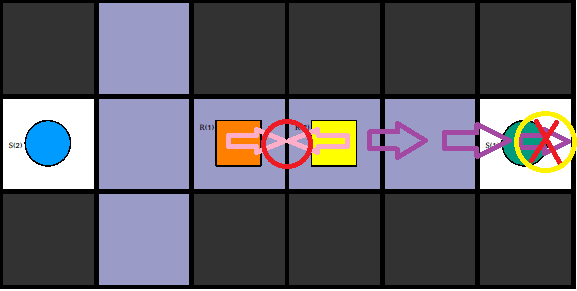
\includegraphics[width=\textwidth, height= 5cm, keepaspectratio]{deadend}}
\end{figure}

Commonly, this happens when a robot, which gets assigned the higher priority for whatever reason is the one which could actually reach a position from where to dodge normally by moving backwards, while the lower priority robot has no such luck. This is best illustrated in figure 4.\newline
In order to deal with this problem, we instituted the predicate deadend/2.\newpage
\begin{lstlisting}[basicstyle=\fontsize{9}{11}\selectfont\ttfamily,frame=single,breaklines=true]
deadend(R1,T) :- dodge_coll(R1,R2,T), back_dodge(R1,T-1), move(R2,D,T,_), position(R1,C1,T-1), not nextto(C1,D,_).
deadend(R2,T) :- dodge_coll(R1,R2,T), back_dodge(R2,T-1), move(R1,D,T,_), position(R2,C2,T-1), not nextto(C2,D,_).
\end{lstlisting}
This rule returns as true as soon as a robot, which had previously been assigned to dodge backwards by back\_dodge/2, moves to a position from where it is unable to move anywhere but the direction it came from in the last step. This will help us in the next variation of back\_dodge/2.
\begin{lstlisting}[basicstyle=\fontsize{9}{11}\selectfont\ttfamily,frame=single,breaklines=true]
back_dodge(R1,T) :- dodge_coll(R1,R2,T), back_dodge(R2,T-1), deadend(R2,T).
back_dodge(R2,T) :- dodge_coll(R1,R2,T), back_dodge(R1,T-1), deadend(R1,T).
\end{lstlisting}
With the help of deadend/2, the new variant rule simply switches around which of the robots has to move backwards, by checking first if a robot had to dodge backwards in the previous step and then if the same robot now encountered a deadend. If that is the case, the other robot begins to dodge backwards instead, and the first robot may move normally again.\newline\newline
One additional scenario may still occur however. Recall both no\_dodge/2 and occ\_dodge/2 dealt with a situation in which only one robot was "allowed" to be unable to dodge, and specifically required that the other (occ\_dodge/2 for no\_dodge/2; no\_dodge/2 for occ\_dodge/2) is not true. With the help of back\_dodge/2 it is now possible to deal with the situation in which both robots are unable to dodge for different reasons.
\begin{lstlisting}[basicstyle=\fontsize{9}{11}\selectfont\ttfamily,frame=single,breaklines=true]
back_dodge(R2,T) :- dodge_coll(R1,R2,T), not dodge_where(R1,_,T), occ_dodge(R2,T).
back_dodge(R1,T) :- dodge_coll(R1,R2,T), not dodge_where(R2,_,T), occ_dodge(R1,T).
\end{lstlisting}
Specifically, if one robot has no valid squares to dodge to, and the other is "merely" blocked by other robots, priority is assigned to the former, as we decided the former is a "more severe" situation that requires immediate dealing with. This way, the robot marked by occ\_dodge/2 will begin dodging backwards for the robot marked by no\_dodge/2.\newline\newline
The last component of back\_dodge is the last variation of dodge\_who/3 we created.
\begin{lstlisting}[basicstyle=\fontsize{9}{11}\selectfont\ttfamily,frame=single,breaklines=true]
dodge_who(R1,D,T) :- move(R2,D,T+1,N), dodge_coll(R1,R2,T), back_dodge(R1,T).
dodge_who(R2,D,T) :- move(R1,D,T+1,N), dodge_coll(R1,R2,T), back_dodge(R2,T).
\end{lstlisting}\newpage
Again conventional priority is done away with, and whichever robot in an edge collision got marked with back\_dodge/2 is forced to "move backwards". This means the robot executes a move in the direction the opponent wishes to go in from the square the dodging robot is currently on. Note that due to copying the move of the opposing robot one step later, rather than the one happening at the same time, it is possible to navigate around corners in a tunnel.

\subsection{Collisions involving Shelves}
We turn now to the topic of the B Domain. Recall that in the B Domain, a robot must be able to navigate to a shelf with an ordered product, carry the shelf to a picking station, deliver the product on the shelf and then return the shelf to its point of origin, all within the given horizon. This requires that our merger be able to deal with collisions caused by shelves as a mobile unit, which introduces a new slew of issues.\newline\newline
The first of these issues arises from the fact that robots are now able to pick up and put down shelves.
\begin{lstlisting}[basicstyle=\fontsize{9}{11}\selectfont\ttfamily,frame=single,breaklines=true]
wait(R2,T) :- move(R2,D,T,N1), pickup(R1,_,T), position(R1,C1,T-1), position(R2,C2,T-1), nextto(C2,D,C1), not nmc_dodge(R2,T).

wait(R2,T) :- move(R2,D,T,N1), putdown(R1,_,T), position(R1,C1,T-1), position(R2,C2,T-1), nextto(C2,D,C1), not nmc_dodge(R2,T).
\end{lstlisting}
Since the act of picking up or putting down a shelf takes a unit of time each to complete, it may happen that a the path of one robot R2 is blocked by another robot R1, which is busy interacting with a shelf. Line 1 specifically checks for the case of pickup, Line 2 for the case of putdown.\newline We judge that the picking up and putting down of shelves takes priority over normal movement actions, therefore robot R2 is ultimately forced to wait until robot R1 has finished its pickup or putdown action. The exact workings of nmc\_dodge/2 and their inclusion here will be explained in their own section. \newline\newline
The next problem that may arise is that a shelf has "gone missing". 
\begin{lstlisting}[basicstyle=\fontsize{9}{11}\selectfont\ttfamily,frame=single,breaklines=true]
wait(R1,T) :- move(R1,D,T,N), step_pickup(R1,S,T+1,N), carries(_,S,T), collision(R1,T-1,N).
\end{lstlisting}
To put it in more precise language, if a robot intends to move to a square where it expects a shelf, which it would pick up in the next time step, but said shelf is already being carried by another robot, it will be forced to hold position for as long as it takes the second robot to properly return the shelf and vacate the spot beneath it.\newpage
\subsubsection{nmc\_dodge/3}\hfill\\
Having considered what possible issues which may arise from a robot intending to pick up or put down a shelf during its normal movement actions, we now take a look at a more exceptional scenario. In it, rather than taking place during normal movements, a robot now interacts with a shelf after having forced another robot, which occupied the spot under the shelf, to dodge out of its way in the previous step.  \newline This way, it blocks the dodging robot from returning to its original square. This is illustrated in figure 5.
\begin{lstlisting}[basicstyle=\fontsize{9}{11}\selectfont\ttfamily,frame=single,breaklines=true]
nmc_dodge(R1,T) :- dodge_who(R1,_,T-1), position(R1,C1,T-1), move(R1,D,T,N1), collision(R1,T-2,N1-1), nextto(C1,D,C2), position(R2,C2,T-1), not move(R2,_,T,N2), collision(R2,T-1,N2).
\end{lstlisting}
nmc\_dodge/2, short for No Move Collision after a dodge, takes care of this issue. 
It checks if a robot was forced to dodge to a position C1 in the previous time step, and then if the return move of move/4 (to recall how the return moves after a dodge work, we recommend taking another look at the chapter on basic dodge moves) is blocked by another robot, which is not following a move command at this time step (which may be because it either is picking up or putting down a shelf). If this turns out to be case, it assigns nmc\_dodge/2 to the robot which dodged.\newline
The next step involves the switching around of its movements.
\begin{lstlisting}[basicstyle=\fontsize{9}{11}\selectfont\ttfamily,frame=single,breaklines=true]
move(R,D,T) :- step_move(R,D,T+1,N), nmc_dodge(R,T), collision(R,T-1,N).

step_move(R,D,T+1,N+1):- step_move(R,D,T,N), nmc_dodge(R,T), collision(R,T-1,N).
\end{lstlisting}
Line 1 inserts into the finished plan the move the robot intended to do after returning from its dodge to the current time step. Line 2 then assigns the "old" return move of the robot to a slot one unit of time later. This means a robot which wanted to move along the X-Axis in order to return to its spot and then along the Y-Axis to continue its movement now instead moves along the Y-Axis first, the X-Axis second. The same applies in case of Y-Axis return, X-Axis continue.\newline
\begin{lstlisting}[basicstyle=\fontsize{9}{11}\selectfont\ttfamily,frame=single,breaklines=true]
step_move(R,D,T1,N+1) :- step_move(R,D,T1,N), nmc_dodge(R,T), collision(R,T-1,N), T1>(T+1), horizon>T1.

step_pickup(R,S,T1,N+1) :- step_pickup(R,S,T1,N), nmc_dodge(R,T),  collision(R,T-1,N), T1>(T+1), horizon>T1.

step_putdown(R,S,T1,N+1) :- step_putdown(R,S,T1,N), nmc_dodge(R,T), collision(R,T-1,N), T1>(T+1), horizon>T1.
\end{lstlisting}
Finally, the existing plans have to be modified again. As the moves of the robot where already pushed back sufficiently when the first edge collision occurred, the only modification happening to the plan after completion of nmc\_dodge/2 is an increase of the collision depth for all moves after it. \newline
\begin{figure}
\floatbox[{\capbeside\thisfloatsetup{capbesideposition={right,top},capbesidewidth=4cm}}]{figure}[\FBwidth]
{\caption{In the previous move, robot 2 dodged for robot 1. Now robot 1 interacts with the shelf and blocks the return of robot 2 (see red circle). Robot 2 will execute its original move instead of the return, moving left, then insert the return move where the original move was cut out, shown with the purple arrows.}\label{fig:test}}
{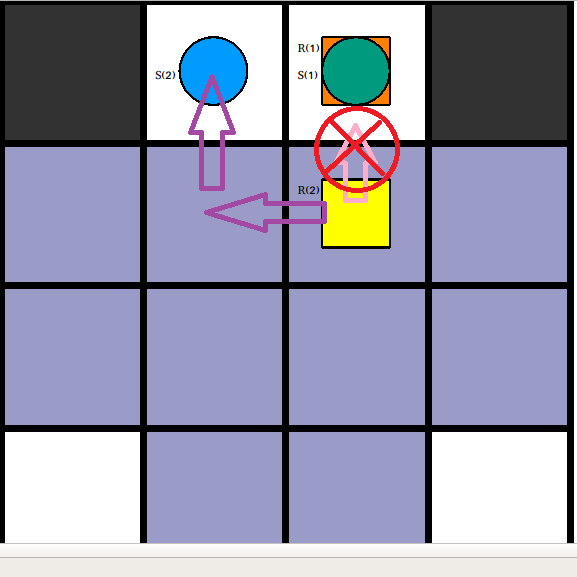
\includegraphics[width=\textwidth, height= 5cm, keepaspectratio]{nmc}}
\end{figure}
\newline
It needs to be noted that this currently only works in situations, in which the return move and the movement of the next time step are not going in the same direction. That means, if both movements are meant to be done along the X-axis or both along the Y-Axis, the program will end up stalling. This will be fixed in a future update, but will not be available for the release copy.\newline
Note also that nmc\_dodge/2 is the product of our earliest designs, before we decided on a unified approach to dodges and waits. We intend to scrap it and insert its functionalities into the wait and dodge rules, but due to time constraints we were not able to do so before the deadline.

\subsubsection{s\_coll/2}\hfill\\
The final issue to be dealt with is that of shelves colliding with one another. Note that this only deals with the collision of a carried shelf with a stationary shelf, as the collisions between two carried shelves are covered by normal robot collision rules.\newline
It is obvious that a robot carrying a shelf, unlike a robot not carrying anything, cannot simple move under a different shelf; it is blocked by the fact that the two shelves would collide. In order to properly catch this, the following predicate was created.
\begin{lstlisting}[basicstyle=\fontsize{9}{11}\selectfont\ttfamily,frame=single,breaklines=true]
s_coll(R,T) :- move(R,D,T,N), position(S2,C2,T-1), position(R,C,T-1), nextto(C,D,C2), carries(R,S,T-1), isShelf(S2), not carries(_,S2,T), not nmc_dodge(R,T), collision(R,T-1,N).
\end{lstlisting}
Rule s\_coll/2 checks if a robot with a shelf has orders to move to a position on which an uncarried shelf, under which no robot is present, stands. It then marks that the carrying robot caused a shelf collision.\newline\newline
What will follow is entirely theoretical at the time of writing. Our intended solution would have been to allow the robot to navigate around the square with the shelf. This would have been done in either one of two ways.\newline In the first, it would move as it would if it had triggered the nmc\_dodge/2 predicate. This would suffice for situations in which the robot would execute a change of directions from the square now blocked by an inert shelf.\newline
In the second, it would again begin as it does in nmc\_dodge/2, but insert additional movements at the end. These would make the robot continue moving past the side of the obstruction, and then insert a move in opposite direction of the first move of nmc\_dodge/2. This would describe an overtaking motion on either the left or right side. \newline\newline
Sadly, due to time constraints we were unable to finish our work on this subject, and had to make do with a bandaid.
\begin{lstlisting}[basicstyle=\fontsize{9}{11}\selectfont\ttfamily,frame=single,breaklines=true]
1{move(R,D,T) : direction(D), D!=D'}1 :- s_coll(R,T), move(R,D',T,N), collision(R,T-1,N).
\end{lstlisting}
This is a bandaid for the simple reason that, if a robot should ever encounter a shelf collision as previously outlined, its plan will be discarded and it is up to the solver itself to find a new one. \newline While this allows us to find solutions which satisfy the goal conditions, in our opinion it goes against the idea of merging and adapting plans to work in concert. As such, we aim to implement a proper solution in a future update.

\newpage


\section{Comparison of Results}
Disclaimer: As our professed goal was not to focus on improving the run time of the merger but rather to challenge it with more complex scenarios and expand it to allow it to work in new problem domains, comparing the run times of the various mergers produced by the different groups in the project is not productive. As such, this section will focus mostly on if and how well our merger solved the 20 benchmarks made available to all for the sake of comparison.\newline
We are of course aware that in a real world scenario, software must be able to fulfill a plethora of demands, of which time efficiency is almost always one. As we were given several distinct choices on which we could focus during this project however, we went with topics that seemed interesting to us. Run time optimization was not one of them.\newline\newline
What will follow is an examination of the results we managed to obtain, split into 5 parts. Each part is dedicated to the benchmarks provided by a different group. Each group provided a total of 4 different benchmarks they deemed interesting. In cases in which a range is given in the horizon, the second number denotes the horizon given by the benchmark creator, while the first number is the lowest possible horizon found by a merger. Horizons in parentheses denote a situation, in which at least on merger decided to override the given horizon of a benchmark. Note that this does not apply to our merger, as we worked solely with the information given by each creator.\newline
Group 1 consists of Adrian, group 2 of Marcus and Max (the authors of this particular report), group 3 consists of Niklas and Marius, group 4 of Tarek and finally group 5 consists of Tom, Hannes and Julian.\newline
Focus will be on those benchmarks that were unsatisfiable for our merger. Please note, only benchmarks a merger successfully returned as unsatisfiable will be denoted as UNSAT in the tables. Cases in which our benchmark took too long to solve were killed by the processor, and are marked instead as "killed".

\subsection{ Benchmarks Group 1}
\begin{table}[]
\begin{tabular}{|c|r|r|r|r|r|c|c|}
\hline
\multicolumn{1}{|l|}{Benchmark} & \multicolumn{1}{l|}{Group 1} & \multicolumn{1}{l|}{Group 2} & \multicolumn{1}{l|}{Group 3} & \multicolumn{1}{l|}{Group 4} & \multicolumn{1}{l|}{Group 5} & Horizon & \multicolumn{1}{l|}{\#Robots} \\ \hline
1                               & 0.027s                  & 0.457s                  & 0.034s                  & 0.058s                  & 0.018s                  & 5       & 2                             \\ \hline
2                               & 0.125s                   & UNSAT                   & 0.017s                  & UNSAT                   & 0.016s                  & 3       & 4                             \\ \hline
3                               & 209.25s                 & 2.903s                  & 0.072s                  & 0.065s                  & 0.094s                  & 7-14    & 2                             \\ \hline
4                               & 55.426s                 & killed                  & 0.179                   & UNSAT                   & UNSAT                   & 9       & 8                             \\ \hline
\end{tabular}
\end{table}
Of the benchmarks of group 1, only the second turns out unsatisfiable for our merger. The reason is the way we have defined our system of priorities within the dodge command. As you recall, if the collision depths of two colliding robots is identical, their ID is taken as tie breaker, with a higher ID having lower priority. In order for the benchmark 2 to be solvable within the given horizon, a robot with a higher ID would have to take priority over a robot with a lower ID in an edge collision in order to not stall the program. However, the case presented in the benchmark does not fall under any of the special edge collision rules we have defined so far and as such results in conflicting orders for robots.\newline
Benchmark 4 on the other hand was killed by the processor after a set amount of time had passed. As our personal analysis of the benchmark found no collision types we did not account for with our established predicates, we are certain that it is solvable provided better hardware.

\subsection{ Benchmarks Group 2}
\begin{table}[]
\begin{tabular}{|c|r|r|r|r|r|c|c|}
\hline
\multicolumn{1}{|l|}{Benchmark} & \multicolumn{1}{l|}{Group 1} & \multicolumn{1}{l|}{Group 2} & \multicolumn{1}{l|}{Group 3} & \multicolumn{1}{l|}{Group 4} & \multicolumn{1}{l|}{Group 5} & Horizon & \multicolumn{1}{l|}{\#Robots} \\ \hline
1                               & 0.032s                  & 0.972s                   & 0.028s                  & 0.029s                  & UNSAT                   & 5-7     & 2                             \\ \hline
2                               & 0.014s                  & 0.105s                  & 0.012s                  & 0.029s                  & UNSAT                   & 4       & 2                             \\ \hline
3                               & 4.949s                  & 6.666s                  & 0.051s                  & 0.041s                  & 0.107s                  & 6-9     & 4                             \\ \hline
4                               & UNSAT                   & 4.578s                  & UNSAT                   & UNSAT                   & UNSAT                   & 15      & 2                             \\ \hline
\end{tabular}
\end{table}
As the benchmarks presented here are those of our own making, it should come as no surprise that our merger was able to solve all of them. Of note is benchmark 4, which is the sole benchmark in the testing group which leaves the M domain and is part of the B domain. As no other group focused on expanding into different domains, it is unsurprising that none of their mergers were able to solve it.

\subsection{ Benchmarks Group 3}
\begin{table}[]
\begin{tabular}{|c|r|r|r|r|r|c|c|}
\hline
\multicolumn{1}{|l|}{Benchmark} & \multicolumn{1}{l|}{Group 1} & \multicolumn{1}{l|}{Group 2} & \multicolumn{1}{l|}{Group 3} & \multicolumn{1}{l|}{Group 4} & \multicolumn{1}{l|}{Group 5} & Horizon & \multicolumn{1}{l|}{\#Robots} \\ \hline
1                               & UNSAT                        & killed                       & 0.902s                       & 0.180s                       & 0.309s                       & 12-17   & 4                             \\ \hline
2                               & 187.834s                     & killed                       & 0.129s                       & 0.418s                       & UNSAT                        & 9       & 8                             \\ \hline
3                               & 6.442s                       & killed                       & 0.229s                       & 0.450s                       & UNSAT                        & 10(12)   & 5                             \\ \hline
4                               & 419.762s                     & killed                       & 0.229s                        & 3.433s                       & UNSAT                        & 21(23)   & 6                             \\ \hline
\end{tabular}
\end{table}
Of the benchmarks provided by group 3, we were sadly unable to produce any satisfactory results due to lack of sufficiently powerful hardware. Again manual analysis leads us to believe that benchmarks 1, 3 and 4 are solvable by our merger in general, as we found no possible collisions we did not account for with the established predicates. This hypothesis is confirmed by the fact that at least one other group was able to successfully run our merger during their tests on these benchmarks and returned results.\newline
Benchmark 2 however is currently beyond our reach. In it, a special type of tunnel collision is described, in which two blocks of robots end up colliding with no ability to dodge out of the way normally, as they are universally blocked on one side by another robot and on the other by a wall. We already outlined that we had not yet covered the scenario where one robot is blocked for two different reasons, which is reason number 1 why our merger will not be able to solve this problem. Reason number 2 is that we also had not yet managed to get back\_dodge/2 to work for cases where more than 2 robots collide in a tunnel, meaning there is no proper translation of the original collision and backwards movement to any robot in a column.

\subsection{ Benchmarks Group 4}

\begin{table}[]
\begin{tabular}{|c|r|r|r|r|r|c|c|}
\hline
\multicolumn{1}{|l|}{Benchmark} & \multicolumn{1}{l|}{Group 1} & \multicolumn{1}{l|}{Group 2} & \multicolumn{1}{l|}{Group 3} & \multicolumn{1}{l|}{Group 4} & \multicolumn{1}{l|}{Group 5} & Horizon & \multicolumn{1}{l|}{\#Robots} \\ \hline
1                               & UNSAT                        & UNSAT                        & UNSAT                        & 0.037s                       & UNSAT                        & 5       & 3                             \\ \hline
2                               & killed                       & UNSAT                        & 0.442s                       & 0.352s                       & UNSAT                        & 19      & 2                             \\ \hline
3                               & 0.350s                       & UNSAT                        & 0.058s                       & 0.191s                       & 0.191s                       & 9(14)    & 3                             \\ \hline
4                               & 1.065s                       & 7.669s                       & 0.084s                       & 0.064s                       & 0.152s                       & 15-16   & 2                             \\ \hline
\end{tabular}
\end{table}
The benchmarks provided by group 4 were the most difficult for our merger. Benchmark 1 turns out unsatisfiable for similar reasons as benchmark 2 of group 3, that being the fact our merger is as yet incapable of properly catching collisions of columns of robots in a tunnel situation. Benchmark 2 is unsatisfiable most likely due to the limitation given by the horizon. The same is true for benchmark 3.

\subsection{ Benchmarks Group 5}

\begin{table}[]
\begin{tabular}{|c|r|r|r|r|r|c|c|}
\hline
\multicolumn{1}{|l|}{Benchmark} & \multicolumn{1}{l|}{Group 1} & \multicolumn{1}{l|}{Group 2} & \multicolumn{1}{l|}{Group 3} & \multicolumn{1}{l|}{Group 4} & \multicolumn{1}{l|}{Group 5} & Horizon   & \multicolumn{1}{l|}{\#Robots} \\ \hline
1                               & UNSAT                        & UNSAT                        & UNSAT                        & 0.047s                       & 0.127s                       & 6-10      & 4                             \\ \hline
2                               & 0.070s                       & 3.000s                       & 0.032s                       & 0.024s                       & 0.060s                       & 4         & 3                             \\ \hline
3                               & killed                       & killed                       & killed                       & UNSAT                        & killed                       & $\sim$40  & 50                            \\ \hline
4                               & killed                       & killed                       & killed                       & UNSAT                        & killed                       & $\sim$100 & 30                            \\ \hline
\end{tabular}
\end{table}
Of the benchmarks of the final group, the first is most interesting, as it fails not for an obvious reason, but rather because unlike every other benchmark, the assignments of robots to shelves is not as our merger expects them. Recall that our goal condition for the M domain demands a robot to be present under a shelf when the horizon is reached, which is checked by comparing the position of a robot with the position of a shelf that shares its ID. This is a quirk that developed mostly due to our habit of assigning robot 1 to shelf 1 and so on. The benchmark in question however assigned shelf 3 to robot 1, shelf 4 to robot 2 etc. Aside from this, no issues with unaccounted for collisions occur. \newline
Due to the sheer size of benchmarks 3 and 4 we were unable to provide a satisfactory result. As their large size is the only "interesting" factor of their design, however, and as such contain no collisions our merger is not equipped to deal with, it is again our belief that neither of them is unsatisfiable given enough time.
\section{Conclusion and Outlook}
\subsection{Conclusions}
The comparison with the mergers of other groups has made several key weaknesses of our own merger obvious. First and foremost is its great time inefficiency, which was to be expected since our focus was on other aspects of the merger. Furthermore, the lack of several features which had to be cut due to time constraints was also keenly felt, such as the inability to deal with multiple robots colliding in a tunnel, as well as the inadequacies of our current priority system for both edge as well as vertex constraints.\newline\newline
On the upside, we are happy to see that most of the problems arising in the unsatisfiable benchmarks were not due to fundamental errors or inabilities of our own merger, but due to constraints imposed by the horizon or due to differences in how plans and instances are laid out. Furthermore, the fact that our merger is the only one presented which is usable not only in the M but the B domain as well, we consider a success.\newline\newline
All in all we believe this first release of our merger was satisfactory, as most of the goals we had set ourselves at the start have been reached. Those goals we had to deprecate to fit the time constraints given by the project lead are discussed in the last section.
\subsection{Outlook}
Here, we will briefly present our plans for future updates.\newline
We plan to modify the predicate occ\_dodge/2 in such a way that it now triggers only if the robots it finds occupying the dodge squares remain there at the time. This way the possibility of "false positives", where the program thinks it found a situation in which occ\_dodge/2 applies, but in reality doesn't, is removed. \newline\newline
Furthermore, we will update back\_dodge/2 to now also take into consideration a situation in which both robots in an edge collision may have triggered an occ\_dodge/2, as well as the situation in which both robots are restricted by both a robot and a wall on either side.\newline\newline
We also intend to integrate nmc\_dodge/2 into the standardized dodge\_who/3 suite of predicates. At the same time it is our intention to expand it, so as to allow it to account for situations in which a robot originally intended to keep moving straight, as currently we are only able to catch exceptions in which the robot switches from moving along the X-Axis to moving along the Y-Axis or vice versa.\newline \newline
In the same vein, another major fix we will be working on relates to the collisions involving one active and one inactive shelf. We will remove the band-aid we have implemented and, most likely taking the changes of nmc\_dodge/2 into account, write concrete rules for dodging around a stationary obstacle.\newline\newline
Last but not least, we have set our sights on expanding into the A domain.



\begin{thebibliography}{1}


\bibitem{url} github repository of the authors, \url{https://github.com/Zard0c/ProjektMAPF}
\bibitem{url} github repository of Adrian Salewsky, \url{https://github.com/salewsky/Plan-Merging}
\bibitem{url} github repository of Niklas Kämmer and Marius Wawerek, \url{https://github.com/NikKaem/mapf-project}
\bibitem{url} github repository of Tarek Ramadan, \url{https://github.com/tramadan-up/asprilo-project}
\bibitem{url} github repository of Tom Schmidt, Julian Bruns and Hannes Weichelt, \url{https://github.com/tzschmidt/PlanMerger}
\bibitem{url} github repository containing the 20 comparison benchmarks described in Section 5 \url{https://github.com/Zard0c/ProjektMAPF/tree/main/working_space/benchmarks}
\bibitem{url} \hypertarget{thesentence}{potassco github repository of asprilo encodings}, \url{https://github.com/potassco/asprilo-encodings/tree/develop}
\bibitem{url} "Experimenting with robotic intra-logistics domains", \url{https://arxiv.org/abs/1804.10247}
\bibitem{url} Figure 1, picture of a generic warehouse environment, taken from the paper "Experimenting with robotic intra-logistics domains", page 7 \url{https://arxiv.org/abs/1804.10247}
\bibitem{url} Figures 2 to 6 taken from benchmarks created by our own group, \url{https://github.com/Zard0c/ProjektMAPF/tree/main/Pictures%20of%20the%20report%2C%20for%20reference}
\end{thebibliography}

\end{document}